\documentclass[a4paper,twoside]{article}
\usepackage[T1]{fontenc}
\usepackage[bahasa]{babel}
\usepackage{graphicx}
\usepackage{graphics}
\usepackage{grffile}
\usepackage{enumitem}
\usepackage{float}
\usepackage[cm]{fullpage}
\pagestyle{myheadings}
\usepackage{etoolbox}
\usepackage{setspace} 
\usepackage{lipsum} 
\setlength{\headsep}{30pt}
\usepackage[inner=2cm,outer=2.5cm,top=2.5cm,bottom=2cm]{geometry} %margin
% \pagestyle{empty}

\makeatletter
\renewcommand{\@maketitle} {\begin{center} {\LARGE \textbf{ \textsc{\@title}} \par} \bigskip {\large \textbf{\textsc{\@author}} }\end{center} }
\renewcommand{\thispagestyle}[1]{}
\markright{\textbf{\textsc{Laporan Perkembangan Pengerjaan Skripsi\textemdash Sem. Ganjil 2018/2019}}}

\onehalfspacing
 
\begin{document}

\title{\@judultopik}
\author{\nama \textendash \@npm} 

%ISILAH DATA BERIKUT INI:
\newcommand{\nama}{Kevin Jonathan}
\newcommand{\@npm}{2014730020}
\newcommand{\tanggal}{11/11/2018} %Tanggal pembuatan dokumen
\newcommand{\@judultopik}{Ant Colony Optimization (ACO) untuk Permasalahan Multi Objective Flowshop Scheduling (MOFSP)} % Judul/topik anda
\newcommand{\kodetopik}{CEN4501}
\newcommand{\jumpemb}{1} % Jumlah pembimbing, 1 atau 2
\newcommand{\pembA}{Cecilia E. Nugraheni}
\newcommand{\pembB}{-}
\newcommand{\semesterPertama}{45 - Ganjil 18/19} % semester pertama kali topik diambil, angka 1 dimulai dari sem Ganjil 96/97
\newcommand{\lamaSkripsi}{1} % Jumlah semester untuk mengerjakan skripsi s.d. dokumen ini dibuat
\newcommand{\kulPertama}{Skripsi 1} % Kuliah dimana topik ini diambil pertama kali
\newcommand{\tipePR}{B} % tipe progress report :
% A : dokumen pendukung untuk pengambilan ke-2 di Skripsi 1
% B : dokumen untuk reviewer pada presentasi dan review Skripsi 1
% C : dokumen pendukung untuk pengambilan ke-2 di Skripsi 2

% Dokumen hasil template ini harus dicetak bolak-balik !!!!

\maketitle

\pagenumbering{arabic}

\section{Data Skripsi} %TIDAK PERLU MENGUBAH BAGIAN INI !!!
Pembimbing utama/tunggal: {\bf \pembA}\\
Pembimbing pendamping: {\bf \pembB}\\
Kode Topik : {\bf \kodetopik}\\
Topik ini sudah dikerjakan selama : {\bf \lamaSkripsi} semester\\
Pengambilan pertama kali topik ini pada : Semester {\bf \semesterPertama} \\
Pengambilan pertama kali topik ini di kuliah : {\bf \kulPertama} \\
Tipe Laporan : {\bf \tipePR} -
\ifdefstring{\tipePR}{A}{
			Dokumen pendukung untuk {\BF pengambilan ke-2 di Skripsi 1} }
		{
		\ifdefstring{\tipePR}{B} {
				Dokumen untuk reviewer pada presentasi dan {\bf review Skripsi 1}}
			{	Dokumen pendukung untuk {\bf pengambilan ke-2 di Skripsi 2}}
		}
		
\section{Latar Belakang}

Penjadwalan produksi merupakan aktivitas yang tidak terpisahkan dalam suatu perusahaan {\it manufakturing}. Penjadwalan ({\it scheduling}) sendiri didefinisikan sebagai suatu proses pengalokasian sumber daya atau mesin-mesin yang ada untuk melaksanakan tugas-tugas yang ada dalam suatu waktu tertentu (Baker, 1974). Sedangkan yang dimaksud dengan proses produksi adalah serangkaian langkah-langkah yang digunakan untuk mentransformasikan {\it Input} menjadi {\it Output}.

Proses penjadwalan {\it Flow Shop} adalah salah satu metode penjadwalan produksi di mana urutan mesin yang digunakan untuk setiap proses dalam seluruh pekerjaan harus sama. Dalam penelitian - penelitian penjadwalan sebelumnya hanya difokuskan pada satu kriteria saja ({\it single}) namun pada penelitian kali ini akan menggunakan lebih dari satu kriteria ({\it multiple}). Banyak algoritma yang dapat digunakan untuk menentukan urutan  pengerjaan pekerjaan dalam proses penjadwalan produksi {\it Flow Shop}. Salah satu algoritma yang dapat digunakan dalam proses penjadwalan produksi {\it Multi Objective Flow Shop} adalah algoritma {\it Ant Colony Optimization}. Algoritma {\it Ant Colony Optimization} adalah algoritma yang mengadopsi perilaku koloni semut yang dikenal sebagai sistem semut. Algoritma ini menyelesaikan permasalahan berdasarkan tingkah laku semut dalam sebuah koloni yang sedang mencari sumber makanan.

Penelitian ini dibuat untuk mempelajari, mengaplikasikan, serta mengukur kinerja Algoritma {\it Ant Colony Optimization} pada proses penjadwalan {\it Multi Objective Flow Shop Scheduling} (MOFSP). Pada skripsi ini juga akan dibuat perangkat lunak yang dapat menerima n job yang masing-masing terdiri atas m buah operasi dan m buah mesin. Setiap operasi hanya ditangani oleh sebuah mesin dan setiap mesin hanya bisa menangani satu operasi. Urutan operasi dari setiap job adalah sama.

\section{Rumusan Masalah}

\begin{enumerate}[label=(\alph*)]
	\item Apa itu penjadwalan {\it Multi Objective Flowshop Scheduling} (MOFSP) ?
	\item Apa itu algoritma {\it Ant Colony Optimization} (ACO) ?
	\item Bagaimana cara kerja dan implementasi algoritma {\it Ant Colony Optimization} (ACO) dalam menyelesaikan permasalahan MOFSP ?
	\item Bagaimana kinerja algoritma {\it Ant Colony Optimization} (ACO) dalam menyelesaikan permasalahan MOFSP ?
	
\end{enumerate}

\section{Tujuan}

\begin{enumerate}[label=(\alph*)]
	\item Menjelaskan penjadwalan {\it Multi Objective Flowshop Scheduling} (MOFSP).
	\item Menjelaskan algoritma {\it Ant Colony Optimization} (ACO) .
	\item Menampilkan  cara kerja dan implementasi algoritma {\it Ant Colony Optimization} (ACO) dalam menyelesaikan permasalahan MOFSP .
	\item Mengetahui kinerja algoritma {\it Ant Colony Optimization} (ACO) dalam menyelesaikan permasalahan MOFSP dengan bantuan {\it benchmark} tertentu.
\end{enumerate}



\section{Detail Perkembangan Pengerjaan Skripsi}
Detail bagian pekerjaan skripsi sesuai dengan rencan kerja/laporan perkembangan terkahir :
	\begin{enumerate}
		\item \textbf{Melakukan studi literatur : penjadwalan proses produksi secara umum, MOFSP, ACO, dan aplikasi ACO untuk masalah penjadwalan.}\\
		{\bf Status :} Ada sejak rencana kerja skripsi.\\
		{\bf Hasil :}
		\begin{itemize}
		\item {\bf Definisi penjadwalan secara umum.}\\
		Secara umum penjadwalan menurut Baker (1974) didefinisikan sebagai proses pengalokasian sumber-sumber dalam    jangka waktu tertentu untuk melakukan sekumpulan pekerjaan. Definisi ini mengandung dua arti yang berbeda, yaitu :
		\begin{enumerate}
		\item Penjadwalan merupakan fungsi pengambilan keputusan, yaitu menentukan jadwal. 
		\item Penjadwalan merupakan suatu teori, yaitu sekumpulan prinsip-prinsip dasar, model-model, teknik-teknik, dan kesimpulan-kesimpulan logis dalam proses pengambilan keputusan yang memberikan dalam fungsi penjadwalan (nilai konseptual).
		\end{enumerate}
		Menurut Conway (1967) Penjadwalan adalah proses pengurutan pembuatan produk secara menyeluruh pada beberapa mesin. Menurut Morton dan Pentico penjadwalan adalah proses pengorganisasian, pemilihan dan pemberian waktu dalam penggunaan sumber dayanya untuk melaksanakan aktivitas yang diperlukan dalam menghasilkan output yang diinginkan dengan memenuhi waktu yang diinginkan pula.
		Persoalan penjadwalan timbul apabila jumlah mesin dan peralatan yang dimiliki terbatas sedangkan terdapat beberapa pekerjaan yang dapat dikerjakan secara bersama. Untuk mendapat hasil yang optimal dengan keterbatasan sumber daya yang dimiliki, maka diperlukan adanya penjadwalan sumber-sumber tersebut secara efisien.
		Tujuan penjadwalan secara umum Baker (1974) adalah :
		\begin{enumerate}
		\item Meningkatkan produktivitas mesin, yaitu dengan mengurangi waktu menganggur mesin.
		\item Mengurangi terhadap persediaan barang setengah jadi, dengan mengurangi rata-rata pekerjaan yang menunggu dalam antrian karena mesin sibuk oleh pekerjaan lain.
		\item Mengurangi keterlambatan (tardiness). Dalam banyak hal, beberapa atau semua pekerjaan mempunyai batas waktu penyelesaian (duedate). Apabila suatu pekerjaan melewati batas waktu tersebut, maka akan dikenai pinalti. Keterlambatan dapat diperkecil dengan mengurangi maksimal tardiness atau mengurangi pekerjaan yang terlambat (number of  tardy job).
		\end{enumerate}
		Pada saat merencanakan suatu jadwal produksi, yang harus dipertimbangkan adalah ketersediaan sumber daya yang dimiliki baik berupa tenaga kerja, peralatan/prosesor ataupun bahan baku. Karena sumber daya yang dimiliki dapat berubah-ubah (terutama operator dan bahan baku), maka penjadwalan dapat kita lihat merupakan proses yang dinamis.
		Masalah penjadwalan muncul karena keterbatasan : 
		\begin{itemize}
		\item Waktu
		\item Tenaga Kerja
		\item Jumlah Mesin
		\item Sifat dan syarat pekerja.
		\end{itemize}
		\end{itemize}
		
		\begin{itemize}
		\item {\bf Klasifikasi Masalah Penjadwalan}\\
		Permasalahan penjadwalan dapat dilihat dari : 
		\begin{enumerate}
		\item Mesin :
		\begin{itemize}
		\item Mesin Tunggal
		\item Mesin ganda (2 mesin)
		\item M mesin
		\end{itemize}
		\item Aliran proses
		\begin{itemize}
		\item {\it Job Shop}
		\item {\it Flow Shop}
		\end{itemize}
		\item Pola Kedatangan
		\begin{itemize}
		\item Statis
		\item Dinamis
		\end{itemize}
		\item Elemen Penjadwalan
		\begin{itemize}
		\item Deterministik
		\item Stokastik
		\end{itemize}
		\end{enumerate}
		
		Metode - metode penyelesaian masalah penjadwalan yaitu : 
		\begin{enumerate}
		\item Heuristic
		\item Matematis
		\item Simulasi
		\end{enumerate}
		\end{itemize}
		
		
		\begin{itemize}
		\item{\bf Penjadwalan {\it Flow Shop}}\\
		Menurut Baker (1974) model penjadwalan dapat dibedakan menjadi 4 jenis keadaan, yaitu :
		\begin{enumerate}
		\item Mesin yang digunakan, dapat berupa proses dengan mesin tunggal atau proses dengan mesin majemuk.
		\item Pola aliran proses, dapat berupa aliran identik atau sembarang.
		\item Pola kedatangan pekerjaan, Statis atau Dinamis.
		\item Sifat informasi yang diterima, dapat berupa Deterministik atau Stokastik.
		\end{enumerate}
		Pada jenis keadaan pertama, jumlah mesin dapat dibedakan atas mesin tunggal dan mesin majemuk. Model mesin tunggal merupakan model dasar dan biasanya dapat diterapkan dalam kasus mesin majemuk.
		Pada model kedua, pola aliran dapat dibedakan atas Flow Shop dan Job Shop. Pada Flow Shop dijumpai pola aliran pemrosesan dari suatu mesin ke mesin yang lain dalam urutan (routing) tertentu. Semua pekerjaan yang mengalir pada saat produksi yang sama tanpa boleh melewatinya disebut dengan pure Flow Shop. Tetapi jika pekerjaan yang datang kedalam Flow Shop tidak harus dikerjakan pada semua mesin, jenis Flow Shop ini disebut dengan General Flow Shop. Contoh pola aliran Pure Flow Shop dan contoh pola aliran Gereral Flow Shop ditunjukkan pada Gambar 1 dan Gambar 2
		
		\begin{figure}[H]
			\centering
			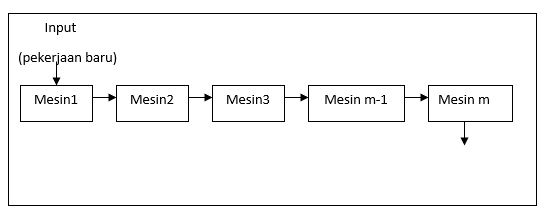
\includegraphics[scale=0.60]{gambar1}
			\caption[Pure Flow Shop] {Pola aliran \it{pure flow shop}}
			\label{fig:pureflowshop}
		\end{figure}
	
	
		\begin{figure}[H]
			\centering
			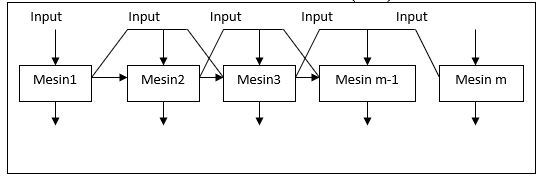
\includegraphics[scale=0.60]{gambar2}
			\caption[General Flow Shop] {Pola aliran \it{general flow shop}}
			\label{fig:generalflowshop}
		\end{figure}
	
		 Pada Job Shop setiap pekerjaan mempunyai routing yang berbeda. Alir proses yang tidak searah ini mengakibatkan setiap pekerjaan yang akan diproses pada suatu mesin dapat merupakan pekerjaan baru atau pekerjaan yang sedang dikerjakan (work in proses).
		 
		\begin{figure}[H]
		 	\centering
		 	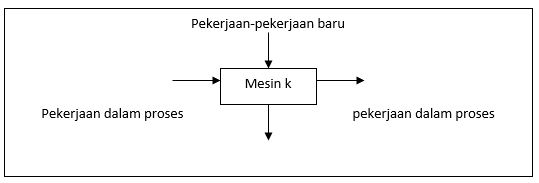
\includegraphics[scale=0.60]{gambar3}
		 	\caption[Job Shop] {Pola aliran \it{job shop}}
		 	\label{fig:jobshop}
		 \end{figure}
		 
		 
		 Pada model ketiga, pola kedatangan pekerjaan dapat dibedakan atas pola kedatangan Statis dan Dinamis. Pada pola Statis, pekerjaan datang secara bersamaan pada waktu nol, siap dikerjakan pada mesin-mesin yang juga sudah siap untuk bekerja atau kedatangan pekerjaan yang tidak bersamaan tetapi saat kedatangan telah diketahui sejak waktu nol. Sedangkan pola Dinamis mempunyai kedatangan pekerjaan tidak menentu, dijumpai adanya variable waktu sebagai faktor pengaruh.
		 
		 Pada model keempat, perilaku elemen-elemen penjadwalan dapat dibedakan atas Deterministik dan Stokastik. Model Deterministik dapat dilihat dari adanya kepastian atas informasi tentang beberapa aspek. Sedangkan pada model Stokastik, mengandung unsur ketidakpastian. Aspek yang dimaksud adalah :
		 \begin{enumerate}
		 	\item Karakteristik pekerjaan dari segi kedatangan, jumlah (kuantitas) pekerjaan, batas waktu penyelesaian (duedate) dan perbedaan kepentingan antar pekerjaan.
		 	\item Karakteristik pekerjaan dari segi banyaknya operasi, susunan mesin dan waktu proses.
		 	\item Karakteristik mesin dari segi jumlah dan kapasitas mesin, kemampuan dan kecocokan tiap mesin dengan pekerjaan yang diberikan. 
		 \end{enumerate}
		Terdapat target utama yang ingin dicapai melalui penjadwalan flow shop ini yaitu jumlah output yang dihasilkan (throughput) berupa makespan. Penjadwalan flow shop didefinisikan sebagai penjadwalan dimana setiap job mempunyai pola aliran atau rute proses yang tetap pada seluruh mesin.
		\end{itemize}	
	
	
		\begin{itemize}
		\item {\bf MOFSP}
		
		\end{itemize}	
		
		\begin{itemize}
		\item{\bf Beberapa Istilah dalam Penjadwalan Flow Shop}\\
		Penjadwalan Flow shop dapat dijelaskan sebagai berikut. Jika terdapat n job $\{j1, j2, \dots\, jn\}$, maka harus diproses pada m mesin $\{m1, m2, \dots, mm\}$. Waktu yang diperlukan untuk memproses job i pada mesin j adalah tij. Jadi permasalahan penjadwalan adalah menentukan urutan job yang memberikan solusi terbaik berdasarkan kriteria tertentu. Beberapa istilah yang digunakan dalam masalah penjadwalan yaitu :
		\begin{enumerate}
		\item Waktu proses (processing time = tj) : yaitu rentang waktu yang dibutuhkan untuk menyelesaikan suatu operasi pada job j.
		\item Ready Time (rj), yaitu saat mulai suatu job j dapat dikerjakan.
		\item DueDate (dj), yaitu batas waktu akhir suatu job harus sudah terselesaikan. Bila melewati batas ini, suatu job dikatakan terlambat (tardy).
		\item Waktu penyelesaian (completion time = Cj) : saat job j telah selesai dikerjakan.
		\item Waktu tinggal (flow time = Fj) : lamanya job j berada dilantai pabrik (shop). Flow time dihitung sejak job siap dijadwalkan sampai job selesai dikerjakan.
		\item Lateness (Lj), yaitu merupakan penyimpangan waktu penyelesaian saat job terhadap duedate job yang bersangkutan. Lateness dihitung dengan persamaan Lj = Cj - dj.
		Lj < 0, saat penyelesaian memenuhi batas akhir (earliness).
		Lj > 0, saat penyelesaian melewati batas akhir (tardiness).
		\item Slack (SLj), yaitu waktu yang tersedia bagi suatu pekerjaan.
		SLj = dj - tj.
		\item Tardiness (Tj), yaitu merupakan keterlambatan penyelesaian suatu job  terhadap duedate job tersebut.
		Tj = max {0,Lj}.
		\item Makespan (Ms), yaitu waktu dimana semua pekerjaan terakhir selesai (MaxLj).
		\end{enumerate}
		\end{itemize}	
		
		\begin{itemize}
		\item{\bf Ant Colony Optimization}\\
		Any Colony Optimization (ACO) awalnya dikembangkan oleh Marco Dorigo et. al. (1996). Algoritma Ant Colony Optimization (ACO) adalah algoritma yang didasarkan pada cara kerja semut untuk menentukan jarak terpendek dari sarang menuju sumber makanan. Semut dapat menemukan jarak terpendek dengan memanfaatkan jejak pheromone (air liur semut) yang dimanfaatkan sebagai komunikasi tidak langsung antar semut. Ketika semut berjalan, ia meninggalkan pheromone dalam jumlah tertentu pada jalur yang dilewatinya. Semut dapat mencium pheromone dan ketika memilih jalur mereka cenderung untuk memilih jalur dengan konsentrasi pheromone yang lebih besar adalah jarak terpendek.
		
		Saat seekor semut yang terisolasi bergerak secara acak, semut ini akan mengikuti jejak yang telah ditinggalkan sebelumnya yang dapat dideteksi dan mempunyai tingkat probabilitas yang tinggi untuk diikuti dan melanjutkan jejak sebelumnya dengan pheromone baru. Tingkah laku kolektif yang muncul disebut dengan tingkah laku Autocalystic, dimana semut yang lain dapat mengikuti jejak yang ada dan jejak yang semakin jelas akan memudahkan bagi semut yang lain untuk mengikutinya. Proses ini secara khusus terjadi melalui kumpulan umpan balik yang positif, dimana kemungkinan semut untuk memilih pola meningkat seiring dengan jumlah semut yang sebelumnya mengikuti pola yang sama.
		
 		\begin{figure}[H]
			\centering
			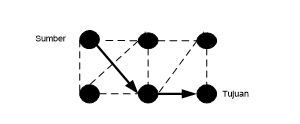
\includegraphics[scale=0.80]{gambar4}
			\caption[Jalur Solusi Semut] {Jalur Solusi Semut {\it Ant Colony Optimization}}
			\label{fig:JaluSolusiSemut}
		\end{figure}
		
		Marco Dorigo et. al. (1996) mengatakan bahwa Ant Colony Optimization adalah algoritma heuristik yang serba guna untuk memecahkan berbagai masalah optimasi. Algoritma ACO memiliki karakteristik sebagai berikut :
		\begin{enumerate}
			\item Serba guna (versatile), dapat dipakai untuk memecahkan masalah dengan versi yang sama, seperti TSP dan Asymetric Travelling Salesman Problem (ATSP).
			\item Sempurna (robust), dapat diterapkan untuk memecahkan dengan hanya perubahan sedikit terhadap masalah optimasi yang lain, seperti Quadratic Assigment Problem dan Job shop Scheduling Problem (JSP).
			\item Pendekatan yang berbasis populasi.
		\end{enumerate}
		\end{itemize}	
		
		\begin{itemize}
		\item {\bf Algoritma Ant Colony Optimization pada penjadwalan flow shop}\\
		Sesuai dengan contoh eksperimen pada gambar 5 terdapat pola saat sekelompok semut berjalan (contoh, dari sumber makanan A ke sarang E, dan sebaliknya). Secara tiba-tiba rintangan muncul dan pola menjadi terpotong. Pada posisi B, semut berjalan dari A ke E (atau pada posisi D yang bergerak dengan arah yang berlawanan) harus memutuskan apakah harus bergerak ke kiri atau ke kanan.
		Pilihan ini dipengaruhi oleh intensitas jejak pheromone yang ditinggalkan oleh semut sebelumnya. Tingkat pheromone yang lebih tinggi pada pola sebelah kanan memberikan semut rangsangan yang lebih kuat dan kemungkinan yang lebih tinggi untuk berbelok ke kanan. Semut pertama mencapai titik B atau D mempunyai kemungkinan yang sama untuk belok ke kiri atau ke kanan (karena tidak terdapat pheromone pada dua pola alternatif tersebut).
		
		Karena pola BCD lebih pendek dibandingkan dengan pola BHD, semut pertama yang mengikuti ini akan mencapai D sebelum semut yang mengikuti pola BHD. Hasilnya adalah semut yang bergerak dari E ke D akan mendapatkan jejak yang lebih jelas pada pola DCB, karena setengah dari semut tersebut yang memilih untuk mendekati rintangan melalui DCBA dan dengan segera akan sampai melalui BCD, mereka akan melalui pola memilih pola DCB dibandingkan pola DHB. Sebagai Konsekuensi, jumlah semut yang mengikuti pola BCD per unit waktu akan lebih banyak dibandingkan dengan jumlah semut yang mengikuti pola BHD.
		
		Hal ini menyebabkan jumlah pheromone pada pola yang lebih pendek akan muncul lebih cepat dibandingkan dengan pola yang lebih jauh, dan oleh karena itu kemungkinan semut yang memilih pola yang diikuti mempunyai bias terhadap pola yang lebih pendek. Hasil akhir yang akan dipilih secara cepat akan ditunjukkan pada pola yang lebih pendek.
		
		Algoritma yang akan dibahas pada bagian selanjutnya adalah model yang berasal dari kumpulan kehidupan nyata semut. Selanjutnya hal ini disebut dengan Sistem Semut dan algoritma yang akan dibahas dikenal dengan algoritma semut. Karakteristik semut asli untuk ketika sedang bergerak dari satu titik ke titik tujuan dapat dilihat pada kedua ilustrasi gambar berikut ini.
		\begin{figure}[H]
			\centering
			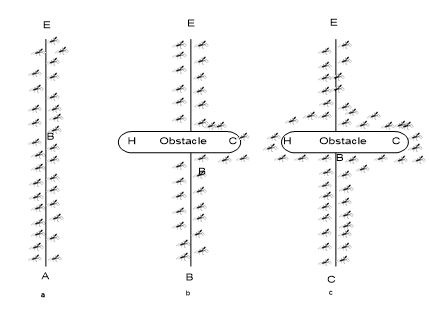
\includegraphics[scale=0.80]{gambar5}
			\caption[Contoh Karakteristik Semut] {Contoh Karakteristik semut}
			\label{fig:karakteristiksemut}
		\end{figure}
		
		
		\end{itemize}
		
		
		
		\item \textbf{Melakukan analisa aplikasi ACO pada masalah MOFSFP.}\\
		{\bf Status :} Ada sejak rencana kerja skripsi.\\
		{\bf Hasil :}

		\item \textbf{Mengembangkan perangkat lunak (analisis, desain, implementasi, dan pengujian).}\\
		{\bf Status :} Ada sejak rencana kerja skripsi.\\
		{\bf Hasil :} Akan dilakukan pada Skripsi 2.
		
	
		\item \textbf{Melakukan eksperimen dengan sebuah {\it benchmark}.}\\
		{\bf Status :} Ada sejak rencana kerja skripsi.\\
		{\bf Hasil :}
		\begin{itemize}
		\item {\bf Data Pengujian}\\
		Dalam melakukan pengujian tingkat keoptimalan dari suatu algoritma, pengujian sebaiknya dilakukan
		dengan menggunakan data kasus standar. Data kasus standar tersebut akan dianggap sebagai
		suatu kasus unik yang memerlukan algoritma khusus untuk proses optimisasinya. Data standar tersebut
		akan digunakan sebagai pembanding dalam proses optimisasi. Dengan menggunakan data
		standar, penilaian kualitas dari suatu algoritma optimisasi dapat dilakukan.
		\end{itemize}
		

		\item \textbf{Menulis dokumen skripsi.}\\
		{\bf Status :} Ada sejak rencana kerja skripsi.\\
		{\bf Hasil :} Berikut ini adalah bagian dari dokumen skripsi yang telah ditulis pada Skripsi 1 : 
		\begin{itemize}
		\item Bab 1
		\item Bab 2
		\item Sebagian Bab 3
		\end{itemize}

	
		

	\end{enumerate}

\section{Pencapaian Rencana Kerja}
Langkah-langkah kerja yang berhasil diselesaikan dalam Skripsi 1 ini adalah sebagai berikut:
\begin{enumerate}
\item Melakukan studi literatur : penjadwalan proses produksi secara umum, MOFSP, ACO, dan aplikasi ACO untuk masalah penjadwalan.
\item Melakukan analisa aplikasi ACO pada masalah MOFSFP.
\item Mempelajari {\it benchmark taliard}.
\item Menulis sebagian dokumen skripsi.
\end{enumerate}




\newpage
\vspace{1cm}
\centering Bandung, \tanggal\\
\vspace{2cm} \nama \\ 
\vspace{1cm}

Menyetujui, \\
\ifdefstring{\jumpemb}{2}{
\vspace{1.5cm}
\begin{centering} Menyetujui,\\ \end{centering} \vspace{0.75cm}
\begin{minipage}[b]{0.45\linewidth}
% \centering Bandung, \makebox[0.5cm]{\hrulefill}/\makebox[0.5cm]{\hrulefill}/2013 \\
\vspace{2cm} Nama: \pembA \\ Pembimbing Utama
\end{minipage} \hspace{0.5cm}
\begin{minipage}[b]{0.45\linewidth}
% \centering Bandung, \makebox[0.5cm]{\hrulefill}/\makebox[0.5cm]{\hrulefill}/2013\\
\vspace{2cm} Nama: \pemB \\ Pembimbing Pendamping
\end{minipage}
\vspace{0.5cm}
}{
% \centering Bandung, \makebox[0.5cm]{\hrulefill}/\makebox[0.5cm]{\hrulefill}/2013\\
\vspace{2cm} Nama: \pembA \\ Pembimbing Tunggal
}
\end{document}

